\documentclass[12pt,letterpaper]{article}
\title{Notes for Experiments with PyTorch}
\author{G H Lathrom}

\usepackage{mystyle}
\usepackage[margin=1in,includehead]{geometry}
\usepackage{wasysym}
\usepackage{tensor}
\usepackage{hyperref}
\usepackage{graphicx}
\usepackage{listings}

\newcommand{\lspan}{\operatorname{span}}
\newcommand{\Ob}{\operatorname{Ob}}
\newcommand{\id}{\operatorname{id}}
\newcommand{\diag}{\operatorname{diag}}
\newcommand{\SO}{\operatorname{SO}}
\newcommand{\Oth}{\operatorname{O}}
\newcommand{\supp}{\operatorname{supp}}
\newcommand{\invlim}{\varprojlim}
\newcommand{\pow}[1]{\operatorname{Pow}\left( #1 \right)}
%\newcommand{\Prob}{\operatorname{Prob}}
\newcommand{\Var}{\operatorname{Var}}
\newcommand{\dunder}[1]{\texttt{\_\_#1\_\_}}

\renewcommand{\theenumi}{\alph{enumi}}

\bibliographystyle{alpha}

\begin{document}
\maketitle


%%%%%%%%%%%%%%%%%%%%%%%%%%%%%%%%%
%%% Header Style
%%%%%%%%%%%%%%%%%%%%%%%%%%%%%%%%%

\pagestyle{fancy}
\fancyhf{}
\lhead{\slshape Machine Learning}
\chead{}
\rhead{\slshape Lathrom}
\fancyfoot[C]{\thepage}
%\renewcommand{\chaptermark}[1]{\markboth{\chaptername \ 
%\thechapter. \ #1}{}} 
\renewcommand{\headrulewidth}{.5pt}
%%%%%%%%%%%%%%%%%%%%%%%%%%%%%%%%%


\section{Multinormal Distributions}

The discussion of this section is largely taken from \cite[Sec.2.5]{multivariate-analysis}.
Taking a real vector space $V$, a bilinear form is a function
\begin{equation*}
	\inner{\cdot,\cdot} : V \times V \ra \bb R
\end{equation*}
which is linear in each of the two components.
Taking the standard basis on $V$, any bilinear form is characterized by an $n\times n$ matrix, $A \in \operatorname{GL}(V) \cong V\otimes V$, as
\begin{equation*}
	\bra{x}A\ket{y} = 
	\begin{bmatrix}
		x^1 & x^2 & \cdots & x^n
	\end{bmatrix} 
	\begin{bmatrix}
		a_{11} & a_{12} & \cdots & a_{1n} \\
		a_{21} & a_{22} & \cdots & a_{2n} \\
		\vdots & \vdots & \cdots & \vdots \\
		a_{n1} & a_{n2} & \cdots & a_{nn} \\
	\end{bmatrix}
	\begin{bmatrix}
		y^1 \\ y^2 \\ \vdots \\ y^n
	\end{bmatrix}
\end{equation*}
Such a bilinear form is said to be \textbf{positive definite} iff
\begin{equation*}
	\bra{x}A\ket{x} > 0 \buf{for all} x \in \bb R^n.
\end{equation*}
It is a well-known property of positive definite matrices that the matrix will be non-singular and the inverse will also be positive definite.  

The multinormal family of distributions is characterized by the parameters $\mu \in \bb R^n$ and $\Sigma$ an $n\times n$ positive definite matrix, that is $N(\mu,\Sigma)$  with pdf given by
\begin{equation*}
	f(x) = \dfrac{1}{\sqrt{2\pi\det(\Sigma)}} \operatorname{exp}\left(-\dfrac 12\bra{x-\mu}\Sigma^{-1}\ket{x-\mu}\right) \buf{for} x \in \bb R^n.
\end{equation*}
The vector $\mu$ is known as the \textbf{mean} vector and $\Sigma$ as the \textbf{covariance} matrix.
Immediate properties of these distributions are that
\begin{equation*}
	\EV[x] = \mu \buf{and} \Var(x) = \Sigma.
\end{equation*}
The regions of equal probability are given by
\begin{equation*}
	\bra{x-\mu}\Sigma^{-1}\ket{x-\mu} = r
\end{equation*}
which are ellipses with major and minor semi-axes corresponding to the principle components or eigenvectors of $\Sigma$.

Generating the data sets was done with the python package \texttt{numpy}, see \cite{harris2020array}.
Two data sets were generated, the first with mean $\mu_1 = \inner{4,4}$ and the second with mean $\mu_2 = \inner{-4,-4}$ while both had covariance matrix
\begin{equation*}
	\Sigma = 
	\begin{bmatrix}
		2 & 1 \\ 1 & 2
	\end{bmatrix}.
\end{equation*}
These were done with the sampling function \\
\indent
\begin{minipage}[t]{.9\textwidth}
\begin{lstlisting}[language=Python]
import numpy as np
import pandas as pd

mu = [4,4]
sigma = [[2,1],[1,2]]
data = np.random.multivariate_normal(mu,sigma, 500)
df1 = pd.DataFrame(data, columns = ['x','y'])
df1['set'] = ['first']*df1.shape[0]
\end{lstlisting}
\end{minipage} \\
The variable \texttt{data} is a $500\times 2$ \texttt{numpy} array which has the form \\
\indent
\begin{minipage}[t]{.9\textwidth}
\begin{lstlisting}[language=Python]
array([[-4.66514356, -3.82006847],
       [-4.29039904, -4.19889765],
       [-3.18884247, -5.95384872],
       [-4.64561036, -5.04998046],
       [-3.1791185 , -1.90862178],
       [-3.89803012, -3.78303282],
\end{lstlisting}
\end{minipage} \\
Figure \ref{fig:data} shows a scatter plot of the data generated by one example run.  The graphs itself were generated using \texttt{plotly} using the following commands \\
\indent
\begin{minipage}[t]{.9\textwidth}
\begin{lstlisting}[language=Python]
import plotly.express as px

df = pd.concat([df1,df2]).reset_index(drop=True)
fig = px.scatter(x=df['x'], y = df['y'], color=df['set'])
fig.show()
\end{lstlisting}
\end{minipage} \\
Our next step is to prepare this data for import into \texttt{PyTorch}.  

\begin{figure}[htpb]
	\begin{center}
		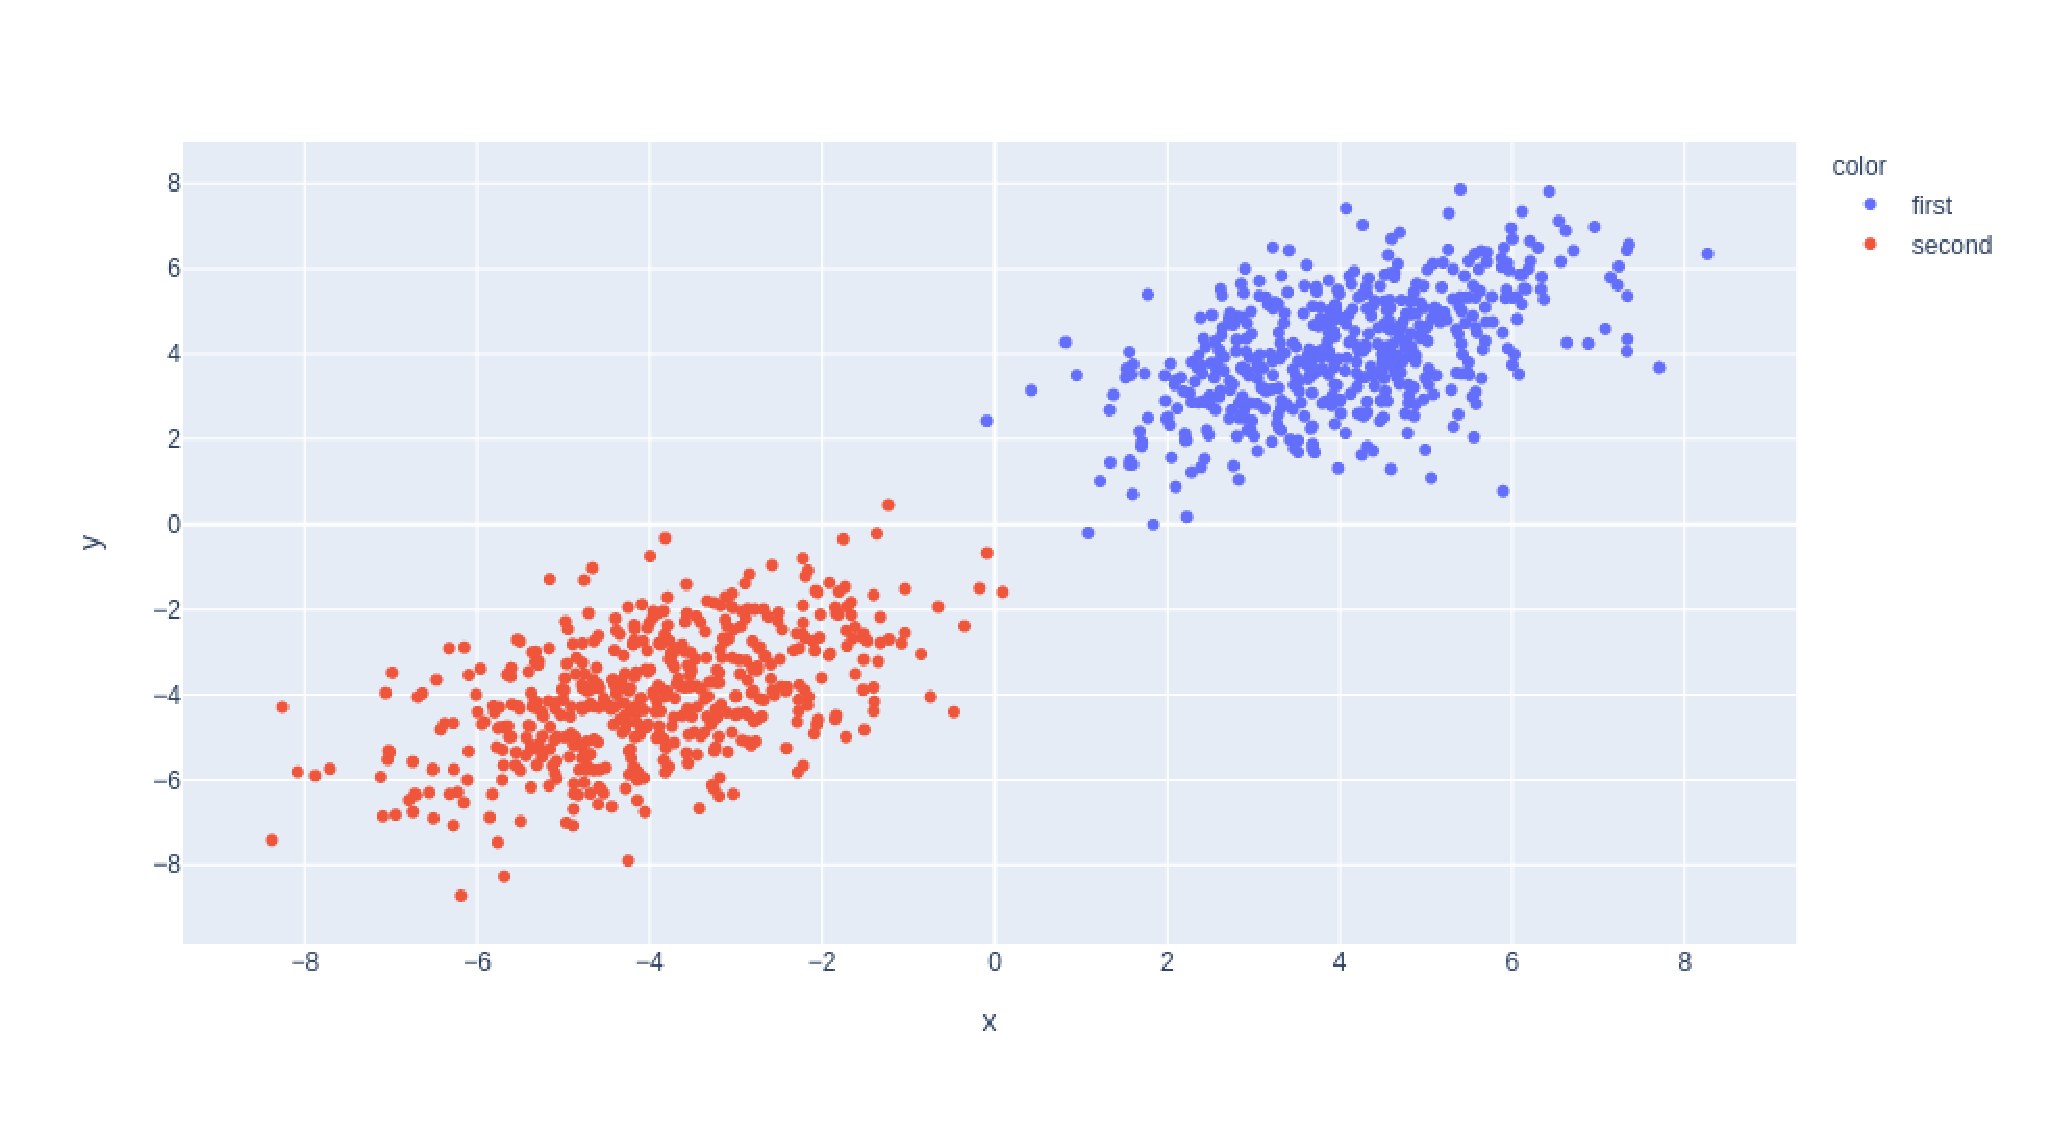
\includegraphics[width=.9\textwidth]{images/data.eps}
	\end{center}
	\caption{Multivariate Examples from Two Data Sets}
	\label{fig:data}
\end{figure}

\section{The \texttt{DataSet} and \texttt{DataLoader} Packages}

The reference used for the PyTorch Documentation is for version 1.7.1 and can be found at \href{https://pytorch.org/docs/1.7.1/}{https://pytorch.org/docs/1.7.1/}.
We load our data as a child class of the \texttt{DataSet} class.  
This class is found in \texttt{torch.utils.data.DataSet} and has two methods which must be overwritten by any child class.  
These are the \dunder{getitem} and \dunder{len} methods. 
These methods do exactly as their names imply, either get a particular data element by index or determine the number of elements in the data set, respectively.

\section{Creating a Linear Discriminator}

\section{Cross-entropy Loss Function}
\cite{wiki:crossentropy}





\bibliography{thebibliography}

\end{document}
